\documentclass[11pt,a4paper]{article}

\usepackage[utf8]{inputenc}
\usepackage[T1]{fontenc}
\usepackage[english]{babel}
\usepackage[a4paper,margin=2.4cm]{geometry}

\usepackage{amsmath, amssymb, amsthm}
\usepackage{mathtools}
\usepackage{booktabs}
\usepackage{tabularx}
\usepackage{array}
\usepackage{caption}
\usepackage{float}
\usepackage{enumitem}
\usepackage{microtype}
\usepackage{xcolor}
\usepackage{listings}
\usepackage{fancyhdr}
\usepackage{titlesec}
\usepackage{graphicx}
\usepackage{tikz}
\usetikzlibrary{positioning, arrows.meta, fit, backgrounds, calc, shapes.geometric}
\usepackage[hidelinks]{hyperref}

%  ---  Palette shared with the companion report  ---
\definecolor{ink}{RGB}{26,30,36}
\definecolor{slate}{RGB}{92,101,112}
\definecolor{mist}{RGB}{233,235,238}
\definecolor{rulegrey}{RGB}{188,194,201}
\definecolor{steel}{RGB}{47,72,102}
\definecolor{steellight}{RGB}{124,146,172}
\definecolor{signal}{RGB}{160,32,45}

\hypersetup{
    colorlinks=true,
    linkcolor=steel,
    citecolor=steel,
    urlcolor=steel,
    pdftitle={The Warehouse Run: An Epistemic Mission over the Amazon Warehouse Floor},
    pdfauthor={Haniel Ulises},
}

\color{ink}

\setlength{\headheight}{22pt}
\pagestyle{fancy}
\fancyhf{}
\fancyhead[L]{\small\textcolor{slate}{\itshape The Warehouse Run}}
\fancyhead[R]{\small\textcolor{slate}{\thepage}}
\renewcommand{\headrulewidth}{0.4pt}
\renewcommand{\headrule}{\hbox to\headwidth{\color{rulegrey}\leaders\hrule height \headrulewidth\hfill}}

\titleformat{\section}{\normalfont\large\bfseries\color{ink}}{\thesection}{0.7em}{}
\titleformat{\subsection}{\normalfont\normalsize\bfseries\color{ink}}{\thesubsection}{0.7em}{}
\titleformat{\paragraph}[runin]{\normalfont\bfseries\color{slate}}{}{0em}{}[.]

\captionsetup{font=small, labelfont={bf,color=slate}, textfont=footnotesize}

\theoremstyle{definition}
\newtheorem{definition}{Definition}

\lstdefinestyle{sys}{
    backgroundcolor=\color{mist},
    basicstyle=\ttfamily\scriptsize\color{ink},
    keywordstyle=\color{steel}\bfseries,
    commentstyle=\color{slate}\itshape,
    stringstyle=\color{slate},
    morecomment=[l]{\#},
    morekeywords={executor,ros__parameters,bt_builder_plugin,bt_node_plugins,
        planner,plan_solver_plugins,EPISTEMIC,conditional_plan,action_mapping,
        Sequence,ReactiveSequence,CheckKnowledge,ApplyEpistemicUpdate,
        EpistemicSwitch,CheckEpistemicGoal,ExecuteAction,true,false,ok,refused},
    frame=single,
    rulecolor=\color{rulegrey},
    framesep=5pt,
    xleftmargin=6pt,
    xrightmargin=0pt,
    breaklines=true,
    showstringspaces=false,
    columns=fullflexible,
    captionpos=b,
}
\lstset{style=sys}

%  ---  Notation  ---
\newcommand{\Ag}{\mathcal{A}}
\newcommand{\Mod}{\mathcal{M}}
\newcommand{\Ev}{\mathcal{E}}
\newcommand{\prd}{\otimes}
\newcommand{\Kop}[1]{K_{#1}}
\newcommand{\Kw}[1]{\mathit{Kw}_{#1}}
\newcommand{\code}[1]{\texttt{\small #1}}


\begin{document}

\begin{titlepage}
\centering
\vspace*{2.4cm}
{\color{rulegrey}\rule{\textwidth}{0.8pt}}\\[0.9cm]
{\LARGE\bfseries The Warehouse Run\par}
\vspace{0.5cm}
{\large\color{slate} The Multi-Robot Amazon Warehouse Exercise,\\ Recast as an Epistemic Domain and Executed on ePlanSys\par}
\vspace{0.7cm}
{\color{rulegrey}\rule{\textwidth}{0.8pt}}\\[1.4cm]

{\large Haniel Ulises\par}
\vspace{0.3cm}
{\color{slate} Epistemic Robotics}\\
\vspace{0.15cm}
{\color{slate}\today}

\vfill
{\color{slate}\small
The RoboticsAcademy multi-robot Amazon warehouse exercise gives a fleet a floor
of racks, a pallet and a dock, and asks for a task planner that assigns the
jobs. It never asks how a robot comes to \emph{know} where the pallet is. Here
that is the whole problem. The floor is that exercise's own, AWS RoboMaker's
small warehouse at its own coordinates, and the plan is not a sequence but a
policy, whose branch is decided by what a laser returns.}
\vspace{1.2cm}
\end{titlepage}

\section{What the exercise leaves out}

The exercise is a good one and it is not about knowledge. Two robots are given
a warehouse, a pallet and a dock; the student writes something that decides who
fetches what, and the robots drive to coordinates they were handed. The
uncertainty a real fleet works under has been removed before the exercise
begins: somebody already knows where the pallet is, and the planner is that
somebody.

Restore the uncertainty and the problem changes shape rather than size. Suppose
the pallet is in one of two aisles and no robot knows which. Then there is no
sequence of actions that delivers it. Every sequence commits, in advance, to an
aisle, and half of them are wrong. What the mission needs is a policy: drive to
a place where the question can be answered, answer it, and continue
accordingly. Producing that requires a planner whose states are not situations
but \emph{sets} of situations an agent cannot tell apart, which is what
epistemic planning is for.

Two further things fall out of restoring it, and both are visible in the run.

\paragraph{A precondition about the robot rather than about the warehouse} A
robot may lift the pallet only where it \emph{knows} the pallet is. Drop that
conjunct and one recovers exactly the classical domain: a robot that happens to
be standing in the right aisle lifts a pallet it has no reason to believe is
there, and a plan that never looks at anything is valid.

\paragraph{A map is what has been measured} The robot starts at shipping with
an empty occupancy grid. The service lane it has to reach is not blocked, it is
\emph{unmeasured}, and a route planner that treats unmeasured floor as free
plans through walls it has not met. This is the same distinction one level
down, and it is answered by the same repository's $\mu$-calculus route planner
rather than by the epistemic one.

This report describes the domain \code{robot-warehouse}, its solution for one,
two and three agents, and its execution in Gazebo on ePlanSys with SLAM and
Nav2 underneath.

\section{The floor}

The grid is not a drawing that resembles the exercise's warehouse. It is
rasterised from the collision meshes Gazebo itself loads for that world (the
building shell, six rack rows, the tall shelf on the west wall and the clutter
between them), sliced at the heights a ground robot can strike. Fourteen
metres by twenty-one at five centimetres a cell: $281 \times 421$.

The two maps AWS ships beside that world were not used. They are SLAM captures:
sparse, noisy, and missing most of the racks, so planning on them would make
every result an artefact of whoever drove the robot the day they were recorded.

One detail of that floor decides the shape of the whole domain. The rack rows
stop $0.15$\,m short of the east wall. To a planner that treats a robot as a
point, that gap is a corridor running the length of the rack block and joining
every aisle to every other; routes down it are routes no TurtleBot could drive,
since the robot is $0.21$\,m across. Growing the obstacles by the robot's
$0.105$\,m radius closes it and leaves $0.7$\,m of each aisle. So in the zone
graph an aisle is a \emph{pocket with one mouth}, and there is no edge from one
bay to the next. That is why a robot that looks into \code{bay2} and finds it
empty has to come back out to the lane, and why the plan pays for that.

\section{The domain}

Six zones: \code{dock\_south} (shipping) and \code{dock\_north} (receiving) at
the two ends of the west \code{corridor}, the service \code{lane} along the
rack fronts, and \code{bay2} and \code{bay3} opening off it. Four propositions
and three rigid facts suffice:

\begin{center}
\begin{tabular}{@{}ll@{}}
\toprule
\code{(at-ag ?i ?z)} & where each robot is \\
\code{(pallet-at ?z)} & which zone the pallet is in \\
\code{(carrying ?i)} & whether \code{?i} has it \\
\code{(delivered)} & whether it has reached a dock \\
\midrule
\code{(adjacent ?z1 ?z2)}, \code{(bay ?z)}, \code{(dock ?z)} & the floor plan, which does not change \\
\bottomrule
\end{tabular}
\end{center}

Driving, lifting and unloading are \emph{public ontic} actions. A warehouse
fleet tracks where its own members are, and the exercise's robots publish
odometry to each other, so a move is common knowledge. Keeping movement public
is what keeps the pallet the only thing in doubt.

Looking is \emph{semi-private sensing}, with one event per answer:

\begin{lstlisting}
(:event e-inspect-found
  :parameters (?i - agent ?z - zone)
  :precondition
    (and (at-ag ?i ?z) (bay ?z) (pallet-at ?z) (<Kw. ?i> (pallet-at ?z))))

(:event e-inspect-empty
  :parameters (?i - agent ?z - zone)
  :precondition
    (and (at-ag ?i ?z) (bay ?z) (not (pallet-at ?z)) (<Kw. ?i> (pallet-at ?z))))

(:action inspect
  :parameters (?i - agent ?z - zone)
  :action-type (semi-private-sensing
    (e-inspect-found ?i ?z)
    (e-inspect-empty ?i ?z))
  :observability-conditions (:and (?i Fully) (default Partially)))
\end{lstlisting}

Semi-private says that the robot which looks learns the answer, while anyone
else present sees it look without learning what it saw. With one robot the
distinction is invisible; modelling it as public would nevertheless be a lie,
and one that stops being harmless the moment a second robot is added. The
\code{<Kw. ?i>} conjunct in both preconditions says the question must be open:
an inspection that settles nothing is not an action, it is a no-op with a cost.

The two events are contradictory, and neither is known to apply when the plan
is built. That is exactly what makes the solution branch.

\subsection{The precondition the domain exists for}

\begin{lstlisting}
(:event e-pickup
  :parameters (?i - agent ?z - zone)
  :precondition
    (and (at-ag ?i ?z) (bay ?z) (pallet-at ?z) ([?i] (pallet-at ?z))
         (not (carrying ?i)))
  :effects (:and (carrying ?i) (not (pallet-at ?z))))
\end{lstlisting}

\code{(pallet-at ?z)} is a claim about the warehouse; \code{([?i] (pallet-at
?z))} is a claim about the robot. Both are required. The first makes lifting
possible, the second makes it \emph{permitted}, and it is the second that the
whole policy is built to establish.

\subsection{The instance}

The ROS demonstration runs \code{instances/problem\_1.epddl}: one robot,
starting at shipping. What the initial state does not say is which bay the
pallet is in. It says only that it is in exactly one of them, and says so as
common knowledge, so the model designates two worlds rather than one:

\begin{lstlisting}
([C. All] (and (or (pallet-at bay2) (pallet-at bay3))
               (not (and (pallet-at bay2) (pallet-at bay3)))
               ...))
(:forall (?i - agent) ([C. All] (<Kw. ?i> (pallet-at bay2))))
(:forall (?i - agent) ([C. All] (<Kw. ?i> (pallet-at bay3))))

(:goal (and (delivered) ([Kw. r1] (pallet-at bay2))))
\end{lstlisting}

The goal asks for two things of different kinds at once. \code{(delivered)} is
ontic and could in principle be had by luck. $\Kw{r_1}\,\mathit{pallet\text{-}at\
bay_2}$ cannot: no amount of moving the pallet satisfies a conjunct under
$\Kw{}$, and only coming to know does. That is what forces the plan to sense.

\section{Grounding and search}

\code{plank} parses and grounds the instance; ALETHEIA, running as ePlanSys's
plan-solver plugin, searches it.

\begin{center}
\begin{tabular}{@{}lr@{}}
\toprule
Atoms & 62 \quad (13 of them rigid facts) \\
Ground actions & 66 \\
Initial worlds & 2, both designated \\
Goal modal depth & 1 \\
Search depth & 11 \\
Nodes expanded & 1\,008 \\
Time to solve & $0.01$\,s standalone; $1.4$\,s through the ePlanSys client \\
\bottomrule
\end{tabular}
\end{center}

The result is a policy of 17 nodes with a single branch point:

\begin{lstlisting}
go_r1_dock_south_lane           [public-ontic]
go_r1_lane_bay2                 [public-ontic]
inspect_r1_bay2                 [semi-private-sensing]
  +-- e-inspect-empty   (not pallet-at_bay2)
      go_r1_bay2_lane, go_r1_lane_bay3, pickup_r1_bay3,
      go_r1_bay3_lane, go_r1_lane_dock_south,
      go_r1_dock_south_corridor, go_r1_corridor_dock_north,
      unload_r1_dock_north                       => goal reached
  +-- e-inspect-found   (pallet-at_bay2)
      pickup_r1_bay2, go_r1_bay2_lane, go_r1_lane_dock_south,
      go_r1_dock_south_corridor, go_r1_corridor_dock_north,
      unload_r1_dock_north                       => goal reached
\end{lstlisting}

Two leaves. A plan with more than one leaf is not a sequence, and which branch
runs is decided by what the robot finds rather than by the planner. Note also
what the empty branch costs: three extra moves, because there is no edge from
\code{bay2} to \code{bay3}. The building charges for a wrong guess.

The product update along that policy is reproduced independently of the
planner, from the model \code{plank} exported and the events it ground, and
checked at every node: each action the planner used must apply, and the goal
must hold at every leaf. The trace and the check are printed by
\code{scenarios/warehouse/tools/show\_plan.py}, which exits non-zero if the two
disagree.

\section{Where the observation comes from}

Nothing in the ROS package decides what was seen. \code{look\_into} faces the
bay, holds the robot there, and ends when the \emph{model} reports
$\Kw{r_1}\,\mathit{pallet\text{-}at\ bay_2}$. What puts that knowledge in the
model is \code{plansys2\_epistemic\_perception}, classifying the two bays over
the occupancy grid \code{slam\_toolbox} has built from the robot's own laser,
and reporting to the epistemic state which of the two events fired.

If the action node decided it, the demonstration would be a puppet show.

One parameter earns its place here. A bay is visible from the service lane
thirty to sixty seconds before the robot reaches it, and the epistemic state
will not accept an observation from a robot it does not yet believe is in the
bay. Perception therefore keeps re-offering the reading until the executor has
applied the drive: \code{applicability\_retries}, set to 240. The default of 40
grids is a few seconds, which fits a building of small rooms and not a
warehouse aisle.

\section{Crossing a floor that is half unmeasured}

\code{goto\_zone} asks the $\mu$-calculus planner for a route and follows it.
It does not plan one. That division is the reason for having both planners:
ePlanSys decides which zone to be in and what must be known there; the
$\mu$-calculus decides how to cross a floor SLAM has only partly filled in, and
refuses, while the way there is unobserved, to cross it at all. Early in a run
the answer is genuinely \emph{no route}, and the log says so:

\begin{lstlisting}
to lane: at (-3.50, -9.30), asked 'lane', 0 legs; 0 cells of lane measured so far
no route to lane yet; going to look from (-1.96, -9.28)
to lane: at (-1.76, -9.03), asked 'lane', 15 legs, and the zone is not on the map yet
to lane: at (0.36, -8.83), asked 'frontier', 24 legs; 285 cells of lane measured
\end{lstlisting}

Standing still is not a reply to that, so when the destination comes back
unreachable the drive picks a \emph{frontier}: a cell that is known free, has
room for the robot and the planner's inflation around it, and has unmeasured
floor within sensor range. It routes to that instead, and asks again. Three
details are load-bearing, and each of them was, at some point, a robot going
nowhere:

\begin{itemize}[leftmargin=1.2em]
\item \textbf{The target must border the unknown.} Score by closeness to the
goal alone and the robot walks to whichever corner of the measured region
points at the destination and stops: the map stops growing and the goal stays
unreachable.
\item \textbf{The score rewards travelling.} Subtracting the distance to the
frontier over known floor is what gets the robot out of a dead end.
\item \textbf{A chosen frontier is committed to until it is reached.} A route
to a frontier succeeds, which clears the no-route flag, which makes the next
cycle ask for the destination, fail, and choose a \emph{different} frontier.
Left alone the robot alternates between two of them and travels nowhere.
\end{itemize}

None of this decides anything epistemic. It is how the robot earns the map that
the $\mu$-calculus planner, and then perception, are entitled to reason about.

\section{Execution}

The world is launched unmodified, a TurtleBot3 burger is spawned at shipping,
and the mission runs end to end. Timings are from the run's own log, relative
to the first action dispatched:

\begin{center}
\begin{tabular}{@{}rll@{}}
\toprule
$t$ (s) & Event & \\
\midrule
$-2$ & \code{problem seeded; asking for a plan} & \\
$-1$ & \code{policy: 17 nodes, 1 of them branching} & \\
$0$ & \code{executing goto\_zone} & shipping $\rightarrow$ lane $\rightarrow$ bay 2 \\
$79$ & \code{executing look\_into} & \\
$79.2$ & \code{(Kw r1 pallet-at\_bay2) holds after 0.4s} & the model settles \\
$80$ & \code{executing pick\_up} & now permitted \\
$84$ & \code{executing goto\_zone} & bay 2 $\rightarrow$ lane $\rightarrow \cdots \rightarrow$ receiving \\
$212$ & \code{executing drop\_off} & \\
$227$ & \code{mission complete: the policy reached its goal} & \\
\bottomrule
\end{tabular}
\end{center}

The found branch was taken: the pallet was in \code{bay2}, so the policy went
straight from \code{look\_into} to \code{pick\_up} without the three extra
moves the empty branch would have cost.

The recording is $76$\,s at $5\times$, $3840 \times 1040$, Gazebo on the left
and RViz on the right, captured on a virtual display. The captions are burned
in by \code{ffmpeg} from the run's own log (the actions ePlanSys dispatched and
the moment the epistemic state settled), so they cannot drift from what the
robot did. The epistemic status in the corner is not narration either: it
is a live \code{EpistemicStateClient::check\_formula} query, and it reads
\code{UNKNOWN} until the robot has looked.

\paragraph{Why the caption is not an RViz marker} An RViz text marker is
geometry in the 3-D scene. It scales with the camera, spaces its words oddly,
and once a 3840-pixel capture is scaled down for viewing it is a row of thin
grey smudges. Several attempts at making it legible that way failed, and they
failed for a reason that was not going to be tuned away.

\section{The fleet, executed}

The two- and three-robot instances were run in the same simulator, and the
execution is not the same shape as the search. Every policy the planner returns
has $r_1$ do the fetching, because $r_1$ is the one that comes on shift at
shipping; what a second and third robot add is the requirement that they come
to \emph{know}, and only the three-robot instance makes that cost an action.

\begin{center}
\begin{tabular}{@{}llllr@{}}
\toprule
Run & Policy & Branch & Announcement & Robots that move \\
\midrule
1 robot & 17 nodes & found & --- & $r_1$ \\
2 robots & 17 nodes & found & none needed & $r_1$ \\
3 robots & 21 nodes & found & none needed & $r_1$, $r_3$ \\
3 robots, pallet moved & 21 nodes & \textbf{empty} & \textbf{$r_1$ radios bay 3} & $r_1$, $r_3$ \\
\bottomrule
\end{tabular}
\end{center}

\paragraph{The branch nobody films} The first three runs take the same leaf.
$r_1$ looks into bay 2, the pallet is there, and it lifts it --- and nothing on
screen distinguishes that from a scripted fetch, which is a fair thing to say
about it. The claim that the plan is a policy is then in the narration rather
than in the behaviour.

Moving the pallet to the other aisle fixes that, and nothing else changes: the
domain, the instance and the goal are untouched, and no component is told. The
run that follows exercises the other leaf, and two things happen on it that
cannot happen on the first.

The first is the backtrack. The racks stop $0.15$\,m short of the east wall,
which is nothing to a robot $0.21$\,m across, so an aisle is a pocket with one
mouth and a wrong guess costs three extra moves.

The second is the announcement, and it is the only place in the whole
demonstration where an agent has to \emph{tell} another agent something.

\begin{lstlisting}
[epistemic_perception_r1] 'bay2' is clear: inspect_r1_bay2 observed e-inspect-empty
[look_action_r1] (Kw r1 pallet-at_bay2) holds after 0.8s
[epistemic_bt] [(look_into r1 bay2)] observed e-inspect-empty
[announce_action_r1] radioing the fleet at bay3
[warehouse_mission] executing announce
...
[warehouse_mission] mission complete: the policy reached its goal
\end{lstlisting}

With two robots the planner spends no announcement, because \code{pickup} is
public and the fleet watching $r_1$ lift the pallet out of a bay already learns
which bay it was. On \emph{this} branch that stops working: what $r_2$ and $r_3$
have to know is about bay 2, watching a lift in bay 3 settles bay 3, and an
absence is not something anyone can watch.

Note also which way the epistemic condition reads at that moment. It becomes
true the instant the bay is found \emph{empty}, because $\Kw{}$ is knowing
whether: coming to know a thing is false is coming to know it.

\paragraph{The robot that never moves} In the two-robot run $r_2$ issues no
action at all --- the log has no lines for it --- and the goal is still about
$r_2$'s knowledge. It comes to know which bay the pallet was in by watching
$r_1$ lift it, without leaving receiving. That is the cheapest way to learn
something, and the planner finds it without being told to look for it.

\section{What is actually running}

\begin{figure}[H]
\centering
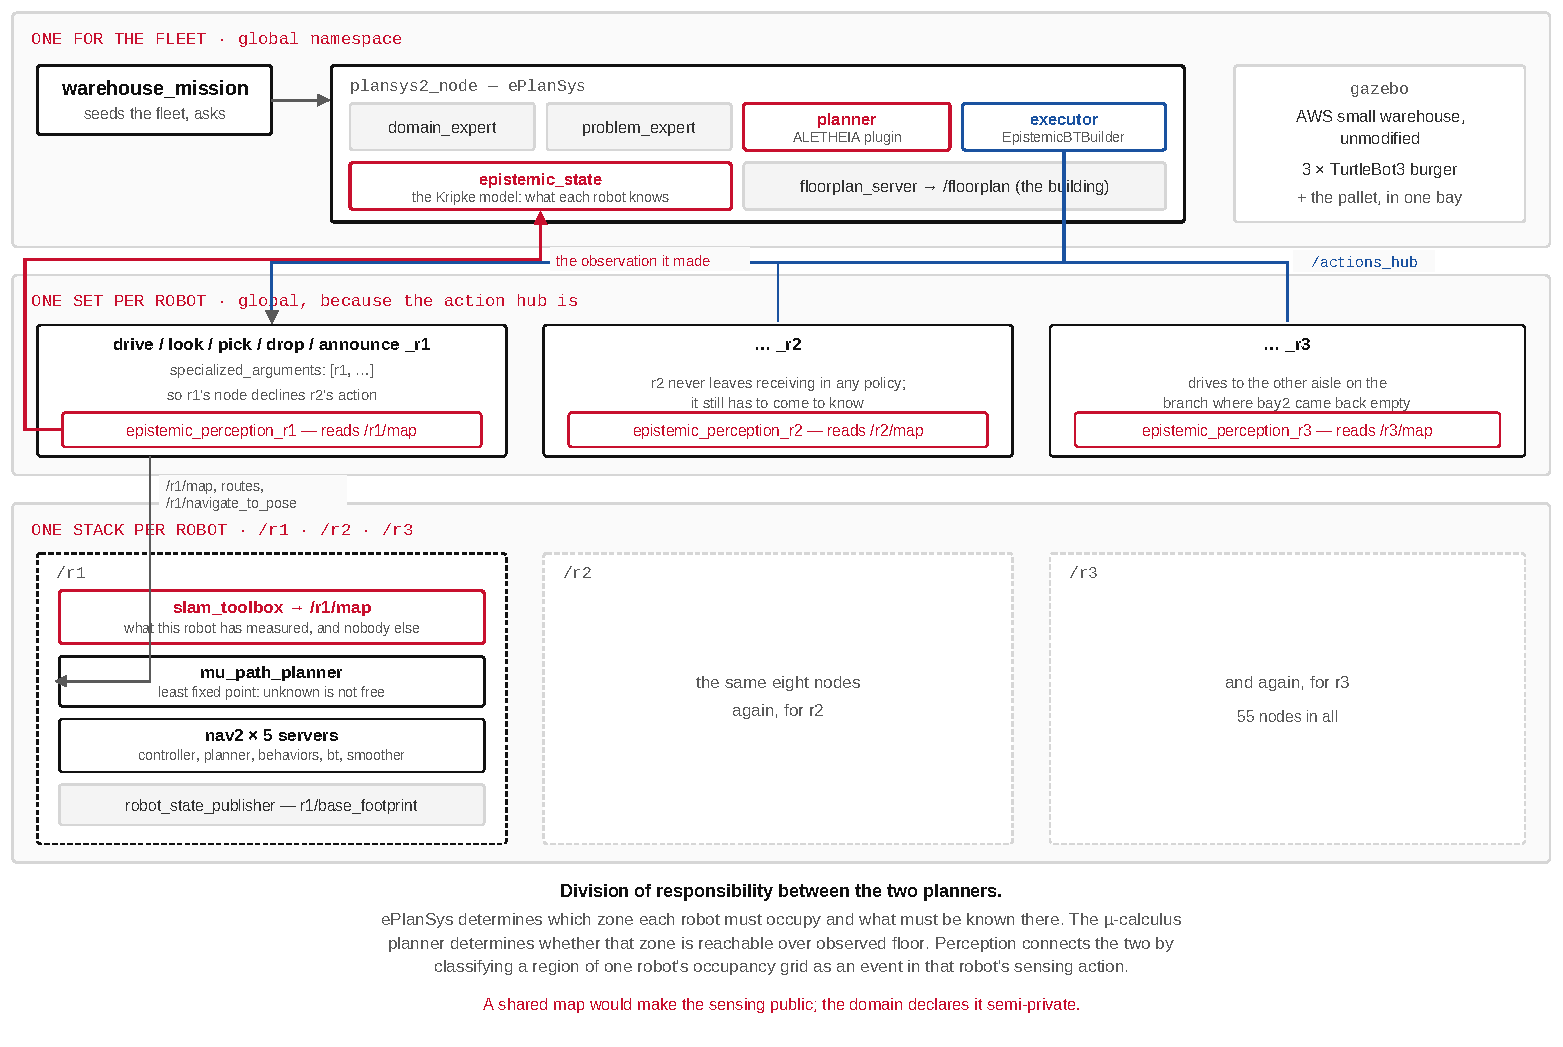
\includegraphics[width=\textwidth]{figures_warehouse_graph.pdf}
\caption{The node graph with three robots. One planning layer for the fleet,
one set of action nodes per robot in the global namespace, and one navigation
stack per robot in a namespace of its own: 55 nodes in all.}
\end{figure}

Where the line falls between those bands is not an arrangement. It is the
difference between what the fleet knows and what one robot has seen, and three
places carry weight.

\paragraph{Each robot maps for itself} Every mapper writes that robot's own
\code{/rN/map}, and its perception node reads only that one. This costs three
SLAM instances and it is not an optimisation to collapse: sensing here is
semi-private, so a shared map would make everything one robot sees immediately
known to all of them, and the demonstration would quietly be proving something
the domain does not say. It is also a trap in the plainest sense ---
\code{slam\_toolbox} names its services relative to the node and its map
\emph{absolutely}, so three mappers in three namespaces all publish the same
\code{/map} until it is remapped by hand.

\paragraph{The action nodes are not namespaced} They cannot be. The executor's
\code{actions\_hub} is a relative name, so a node inside a robot's namespace
advertises its own hub and never hears the fleet's. They run in the global
namespace and decline each other's work through
\code{specialized\_arguments}, which the executor matches positionally against
the action's own arguments.

\paragraph{The building is shared and the map is not} Nav2 plans over
\code{/floorplan}, the rasterised AWS world, served once for the fleet: a
warehouse robot is given the building. What it is not given is a record of what
it has looked at, and that is the per-robot \code{/rN/map} that the
$\mu$-calculus planner and perception both reason over.

\section{What it costs to add a robot}

The two-agent instance moves the epistemic conjunct to the robot that never
leaves receiving: $\mathit{delivered} \wedge
\Kw{r_2}\,\mathit{pallet\text{-}at\ bay_2}$. The three-agent instance asks it of
$r_2$ and $r_3$, neither of whom goes to look.

\begin{center}
\begin{tabular}{@{}rrrrrrrr@{}}
\toprule
Agents & Atoms & Ground actions & Worlds & Depth & Expanded & Generated & Seconds \\
\midrule
1 & 62 & 66 & 2 & 11 & 1\,008 & 1\,012 & 0.01 \\
2 & 69 & 132 & 2 & 11 & 18\,254 & 18\,525 & 0.23 \\
3 & 76 & 198 & 2 & 12 & 195\,178 & 197\,533 & 2.90 \\
\bottomrule
\end{tabular}
\end{center}

Nodes expanded grows by roughly an order of magnitude per robot ($\times 18$,
then $\times 11$). The \emph{mission} does not get harder: the plan is the same
shape and $r_1$ still does all the walking. The search does. Every agent is
another relation over the worlds, and a formula about what somebody knows has
to be checked against all of them.

\paragraph{The announcement the planner declines to make} The two-agent policy
contains no announcement, although the domain offers \code{report-pallet-at}.
It does not need one: \code{pickup} is public, so the fleet seeing $r_1$ lift
the pallet out of a bay is already enough for $r_2$ to know which bay it was.
Add a third robot who must also know and the planner does spend an action on
it, inserting \code{report-pallet-at\_r1\_bay3} on the branch where $r_1$ found
\code{bay2} empty, because there the knowledge comes from an absence, and
watching a lift in \code{bay3} settles \code{bay3}, not \code{bay2}. This is
not something the domain was written to demonstrate; it is what the search
found.

\section{Two rejections}

Both are checked by \code{plank validate}, and both are the expected result.

\paragraph{A sequence, where a policy is needed} Handing the planner the
straight-line sequence that assumes the pallet is in \code{bay2} is rejected:
it is unexecutable in the world where the pallet is in \code{bay3}, which the
agent cannot rule out.

\paragraph{Picking up without looking} \code{pickup\_r1\_bay2}, after driving
to the lane and in to \code{bay2}, is refused, with
\code{false (pickup\_r1\_bay2 is not applicable ...)}, because
$[r_1]\,\mathit{pallet\text{-}at\ bay_2}$ does not hold. Delete that conjunct
from \code{e-pickup} and the same sequence becomes valid, which is exactly the
classical domain this one is not.

\section{Reproducing}

\begin{lstlisting}
# one, two and three agents; the two rejections; the scaling table
bash epddl-workspace/robot-warehouse/validate.sh

# the floor, the six mu-calculus cases, offline and over ROS
colcon build --packages-select epistemic_msgs mu_path_planner warehouse_scenario
bash scenarios/warehouse/run_demo.sh
colcon test --packages-select warehouse_scenario     # 12 tests

# the full system in Gazebo
ros2 launch warehouse_demo warehouse_demo_launch.py
\end{lstlisting}

The domain and its instances are in \code{epddl-workspace/robot-warehouse}; the
floor, its rasteriser and the route-planning cases are in
\code{scenarios/warehouse}; the ROS side, meaning the action nodes, the
parameters, the Nav2 configuration and the launch file, is in
\code{ros2\_ws/src/warehouse\_demo}.

\end{document}
